\chapter{Những công trình liên quan}
Như đã nhắc tới trước đó, các công trình về dự đoán xu hướng giá trị Bitcoin 
hầu như chưa có hoặc chưa được công khai vì thế mà việc tiếp cận chính xác vấn 
đề là điều không thể. Thay vào đó chúng ta sẽ đi sử dụng các vấn đề liên quan 
khác như là dự đoán xu hướng giá trị vàng và dự đoán xu hướng giá trị cổ phiếu.
Hai công trình cụ thể được tham khảo trong luận văn là: 
``Predicting Gold Prices'' \cite{PredictingGoldPrices} và 
``Machine Learning in Stock Price Trend Forecasting'' 
\cite{StockPriceTrendForecasting} \\\\ 
Bài báo \cite{PredictingGoldPrices} liên quan đến ứng dụng Máy học cho việc dự đoán 
giá vàng, tác giả đã chọn hướng tiếp cận học có giám sát và cụ thể là bài toán 
phân lớp. Tập dữ liệu mà tác giả sử dụng là tập dữ liệu giá vàng từ đầu năm 2007 
đến cuối năm 2013 với khoảng 1700 mẫu và được lấy từ trang web của USA Gold, 
đồng thời sử dụng hai giải thuật phân lớp là SVM và LR.
Trong đó, khi gặp phải vấn đề mất cân đối trong tập dữ liệu (nhãn $positive$ 
lớn hơn rất nhiều sao với nhãn $negative$) tác giả đã sử dụng giải thuật SVM 
với nhiều lần điều chỉnh mô hình như: sử dụng kernel RBF, sử dụng kernel tuyến 
tính với L1,... nhưng đều cho ra kết quả thấp (Accuracy nằm trong khoảng 50\% 
- 51\%). Với kết quả như vậy, tác giả đã quyết định sử dụng SVM như một giải 
thuật dùng để so sánh và đánh giá với giải thuật còn lại. Với một hướng tiếp 
cận khác, LR được sử dụng để giải quyết bài toán, kết quả được ghi nhận như 
bảng sau.
\begin{table}[h]
\centering
\begin{tabular}{ |c|c| }
\hline
Precision & 69.90\% \\
\hline
Recall & 72.31\% \\
\hline
Accuracy & 69.30\% \\
\hline
\end{tabular}
\caption{Bảng đánh giá - Predicting Gold Prices}
\end{table}\\
Với kết quả trên, các tham số đánh giá cho kết quả trong khoảng gần bằng 70\% 
và tác giả xem đây là một kết quả có ý nghĩa.\\\\
Bài báo \cite{StockPriceTrendForecasting} liên quan đến ứng dụng Máy học cho việc 
dự đoán giá trị cổ phiếu (cụ thể là công ty 3M), nguồn dữ liệu được sử dụng là 
Bloomberg Data Terminal với khoảng 1400 mẫu. Nhóm tác giả đã sử dụng bốn 
giải thuật trong quá trình phân tích và giải quyết bài toán đó là: GDA, LR, SVM, 
QDA.\\\\
Ngoài ra, tìm ra một hướng giải quyết tối ưu, nhóm tác giả tiếp cận vấn đề dựa 
trên hai mô hình. Thứ nhất, mô hình Ngày tiếp theo (Next-Day Model) với mục 
tiêu đi dự đoán xu hướng giá trị của cổ phiếu trong ngày tiếp theo. Và thứ hai, 
mô hình Dài hạn (Long-Term Model) với mục tiêu đi dự đoán xu hướng giá trị của 
$n$ ngày tiếp theo.\\\\
Kết quả đánh giá của 4 giải thuật cho mô hình Ngày tiếp theo:
\begin{table}[h]
\centering
\begin{tabular}{ |c|c|c|c|c| }
\hline
Model & LR & GDA & QDA & SVM \\
\hline
Accuracy & 44.5\% & 46.4\% & 58.2\% & 55.2\% \\
\hline
\end{tabular}
\caption{Bảng đánh giá mô hình Ngày tiếp theo }
\end{table}\\
Đồ thị đánh giá của 4 giải thuật cho mô hình Dài hạn:
\begin{figure}[h!]
\centering
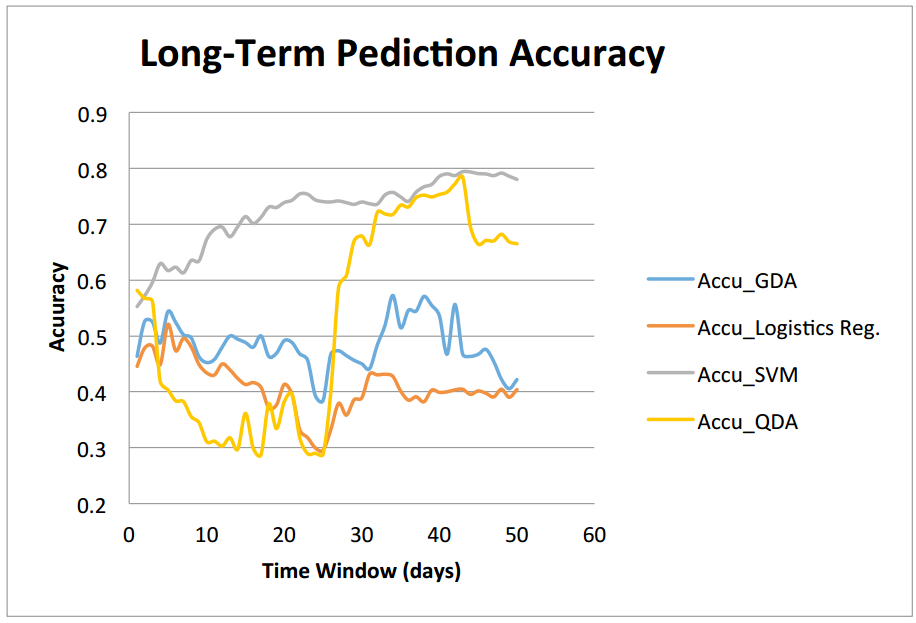
\includegraphics[height=3.5in, keepaspectratio=true]{longtermmodel.png}
\caption{Đồ thị đánh giá mô hình Dài hạn}
\end{figure}\\
Hai mô hình với hai kết quả, ta thấy ở mô hình Dài hạn hai giải thuật SVM và 
QDA cho kết quả Accuracy gần bằng 80\% với $n=44$ ngày, so sánh với mô hình 
Ngày tiếp theo Accuracy gần bằng 60\% ta có thể thấy mô hình dài hạn cho kết 
quả có ý nghĩa hơn. Nhưng một hạn chế rất lớn của công trình này, nhóm tác giả 
chỉ sử dụng một tham số đánh giá duy nhất là Accuracy mà bỏ qua Precision và 
Recall. Việc đánh giá chỉ dựa trên duy nhất một tham số sẽ không thể tổng quát 
được kết quả đầu ra, vì vậy mà dẫn đến nguy cơ không phát hiện các vấn đề về 
lệch dữ liệu hoặc overfitting.\\\\ 
Tổng quan qua hai công trình và tham khảo một số công trình khác, nhận thấy 
đa số các hướng tiếp cận đều đi theo một phương pháp tổng quát chung, nó bao gồm các bước 
cơ bản như:
\begin{enumerate}
\item Xây dựng không gian vector thuộc tính phù hợp với tính chất bài toán
\item Sử dụng các giải thuật phân lớp điển hình trong Máy học như là 
SVM, LR ...
\item Đánh giá giải thuật bằng các tham số Accuracy, Recall, Precision.
\end{enumerate}
Từ những đục kết trên, bản thân nhận thấy các bước trên cũng chính là phương pháp 
nên dùng để tiếp cận đề tài. Ngoài ra, nhận thấy ở hai công trình trên chưa 
hề sử dụng một giải thuật rất được phổ biến hiện nay, nó nổi lên như một đại 
diện của Học sâu - Deep Learning đó là MNN. Do đó mà luận văn này sẽ sử dụng 
MNN như là một giải thuật bổ sung trong quá trình so sánh và đánh giá so với 
các giải thuật phân lớp khác.